\documentclass{article}
\usepackage[margin=1in]{geometry}
\usepackage{problemset}
\showsolntrue

% Custom commands
\newcommand{\R}{\mathbb{R}}
\newcommand{\X}{\mathcal{X}}
\newcommand{\Y}{\mathcal{Y}}
\newcommand{\E}{\mathbb{E}}
\newcommand{\V}{\text{Var}}
\renewcommand{\P}{\mathbb{P}}

\begin{document}

\pstitle{%
    MATH 189%
}{
    Homework 5%
}[due Wednesday, February 25 at 8:00AM]

\textbf{Resources:} These problems appear in Chs. 8-9 of the textbook pgs. 363-366 and 395-398.

\textbf{Format requirements:} Type your homeworks using LATEXwith embedded plots for the applied exercises.

\textbf{Grading:} The grading is based 50\% on completion and 50\% on correctness.

\vspace{1em}

\begin{probset}

% --- Problem 1 ---
\begin{prob}[\textbf{Ch. 8 conceptual exercise 2}] 
    Boosting using depth-one trees (or stumps) leads to an additive model: that is, a model of the form $$f(x) = \sum_{j=1}^p f_j(x_j)$$ Explain why this is the case.

    \begin{soln}
        This is because the depth-one trees are essentially decision stumps, which are just binary splits on a single feature. So each stump's output can be written as $f_j(x_j)$ for some $j$. When we group stumps by the feature they split on, the model becomes $f(x) = \sum_{j=1}^p f_j(x_j)$ where $f_j(x_j)$ is the sum of contributions from stumps that split on feature $j$. Because each term depends on only one variable, there are no interaction terms, so the model is additive in the features.
    \end{soln}
\end{prob}

% --- Problem 2 ---
\begin{prob}[\textbf{Ch. 8 conceptual exercise 6}]
    Provide a detailed explanation of the algorithm that is used to fit a regression tree.

    \begin{soln}
        The steps for fitting a regression tree are as follows:
        \begin{enumerate}
            \item \textbf{Growing:} Recursively split the data into two subsets. For each region, search over all features $j$ and all possible cutpoints $s$, and choose the pair $(j, s)$ that minimizes:
            \[ 
                \sum_{i: x_{ij} < s} (y_i - \hat y_{R_1})^2 + \sum_{i: x_{ij} \geq s} (y_i - \hat y_{R_2})^2
            \]
            where $\hat y_{R_1}$ and $\hat y_{R_2}$ are the mean of the response values in the left and right subsets, respectively. Repeat until a stopping criterion is met (e.g., minimum number of observations per node) to obtain a large tree $T_0$.
            \item \textbf{Pruning:} Prune the tree $T_0$ by finding a subtree $T \subset T_0$ that minimizes:
            \[
                \sum_{m=1}^{|T|} \left( \sum_{i: x_i \in R_m} (y_i - \hat y_{R_m})^2 \right) + \alpha |T|
            \]
            where $\alpha$ is a tuning parameter (typically chosen via cross-validation), $|T|$ is the number of terminal nodes in the tree, and $R_m$ is the region of the $m$th terminal node.
        \end{enumerate}
    \end{soln}
\end{prob}

\newpage

% --- Problem 3 ---
\begin{prob}[\textbf{Ch. 9 conceptual exercise 2}]
    We have seen that in p = 2 dimensions, a linear decision boundary takes the form $\beta_0 + \beta_1X_1 + \beta_2X_2 = 0$. We now investigate a non-linear decision boundary.

    \begin{subprobset}
        \begin{subprob}
            Sketch the curve $(1 + X_1)^2 + (2 - X_2)^2 = 4$.

            \begin{soln}
                \begin{center}
                    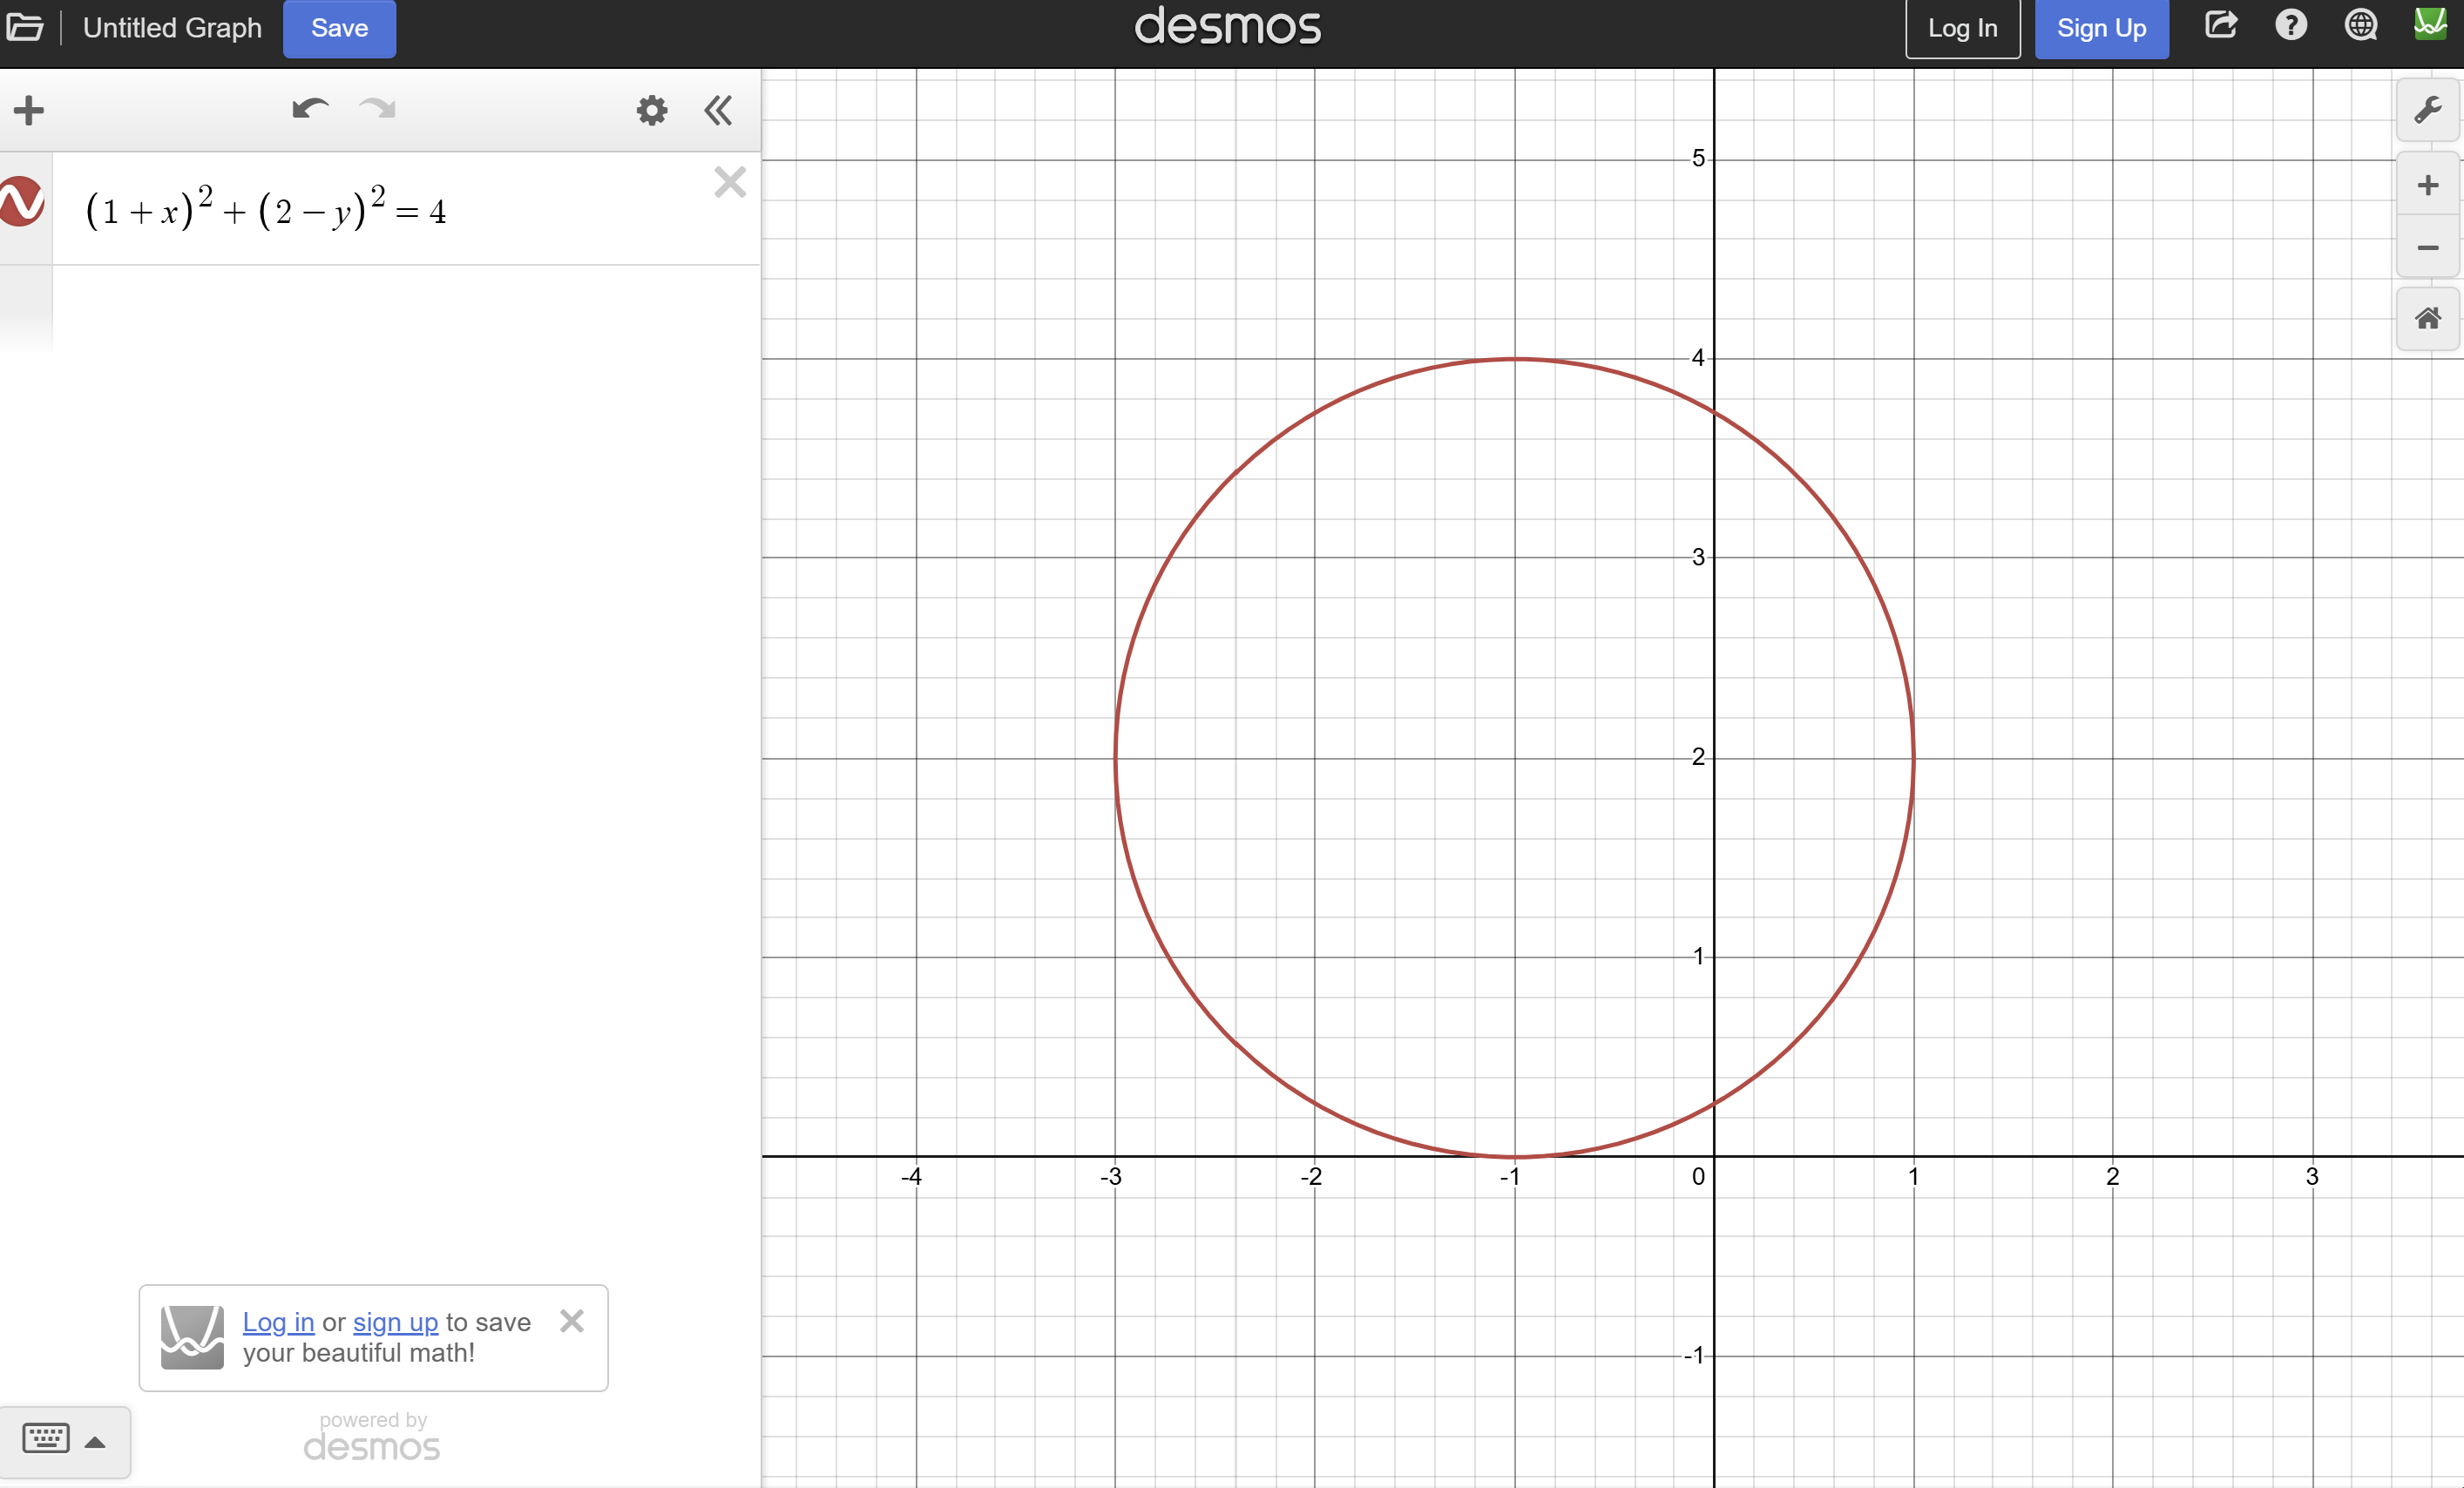
\includegraphics[width=0.5\textwidth]{Images/3a.png}
                \end{center}
                This is a circle centered at $(-1, 2)$ with radius 2.
            \end{soln}
        \end{subprob}

        \begin{subprob}
            On your sketch, indicate the set of points for which $(1 + X_1)^2 + (2 - X_2)^2 > 4$, as well as the set of points for which $(1 + X_1)^2 + (2 - X_2)^2 \leq 4$.

            \begin{soln}
                \begin{center}
                    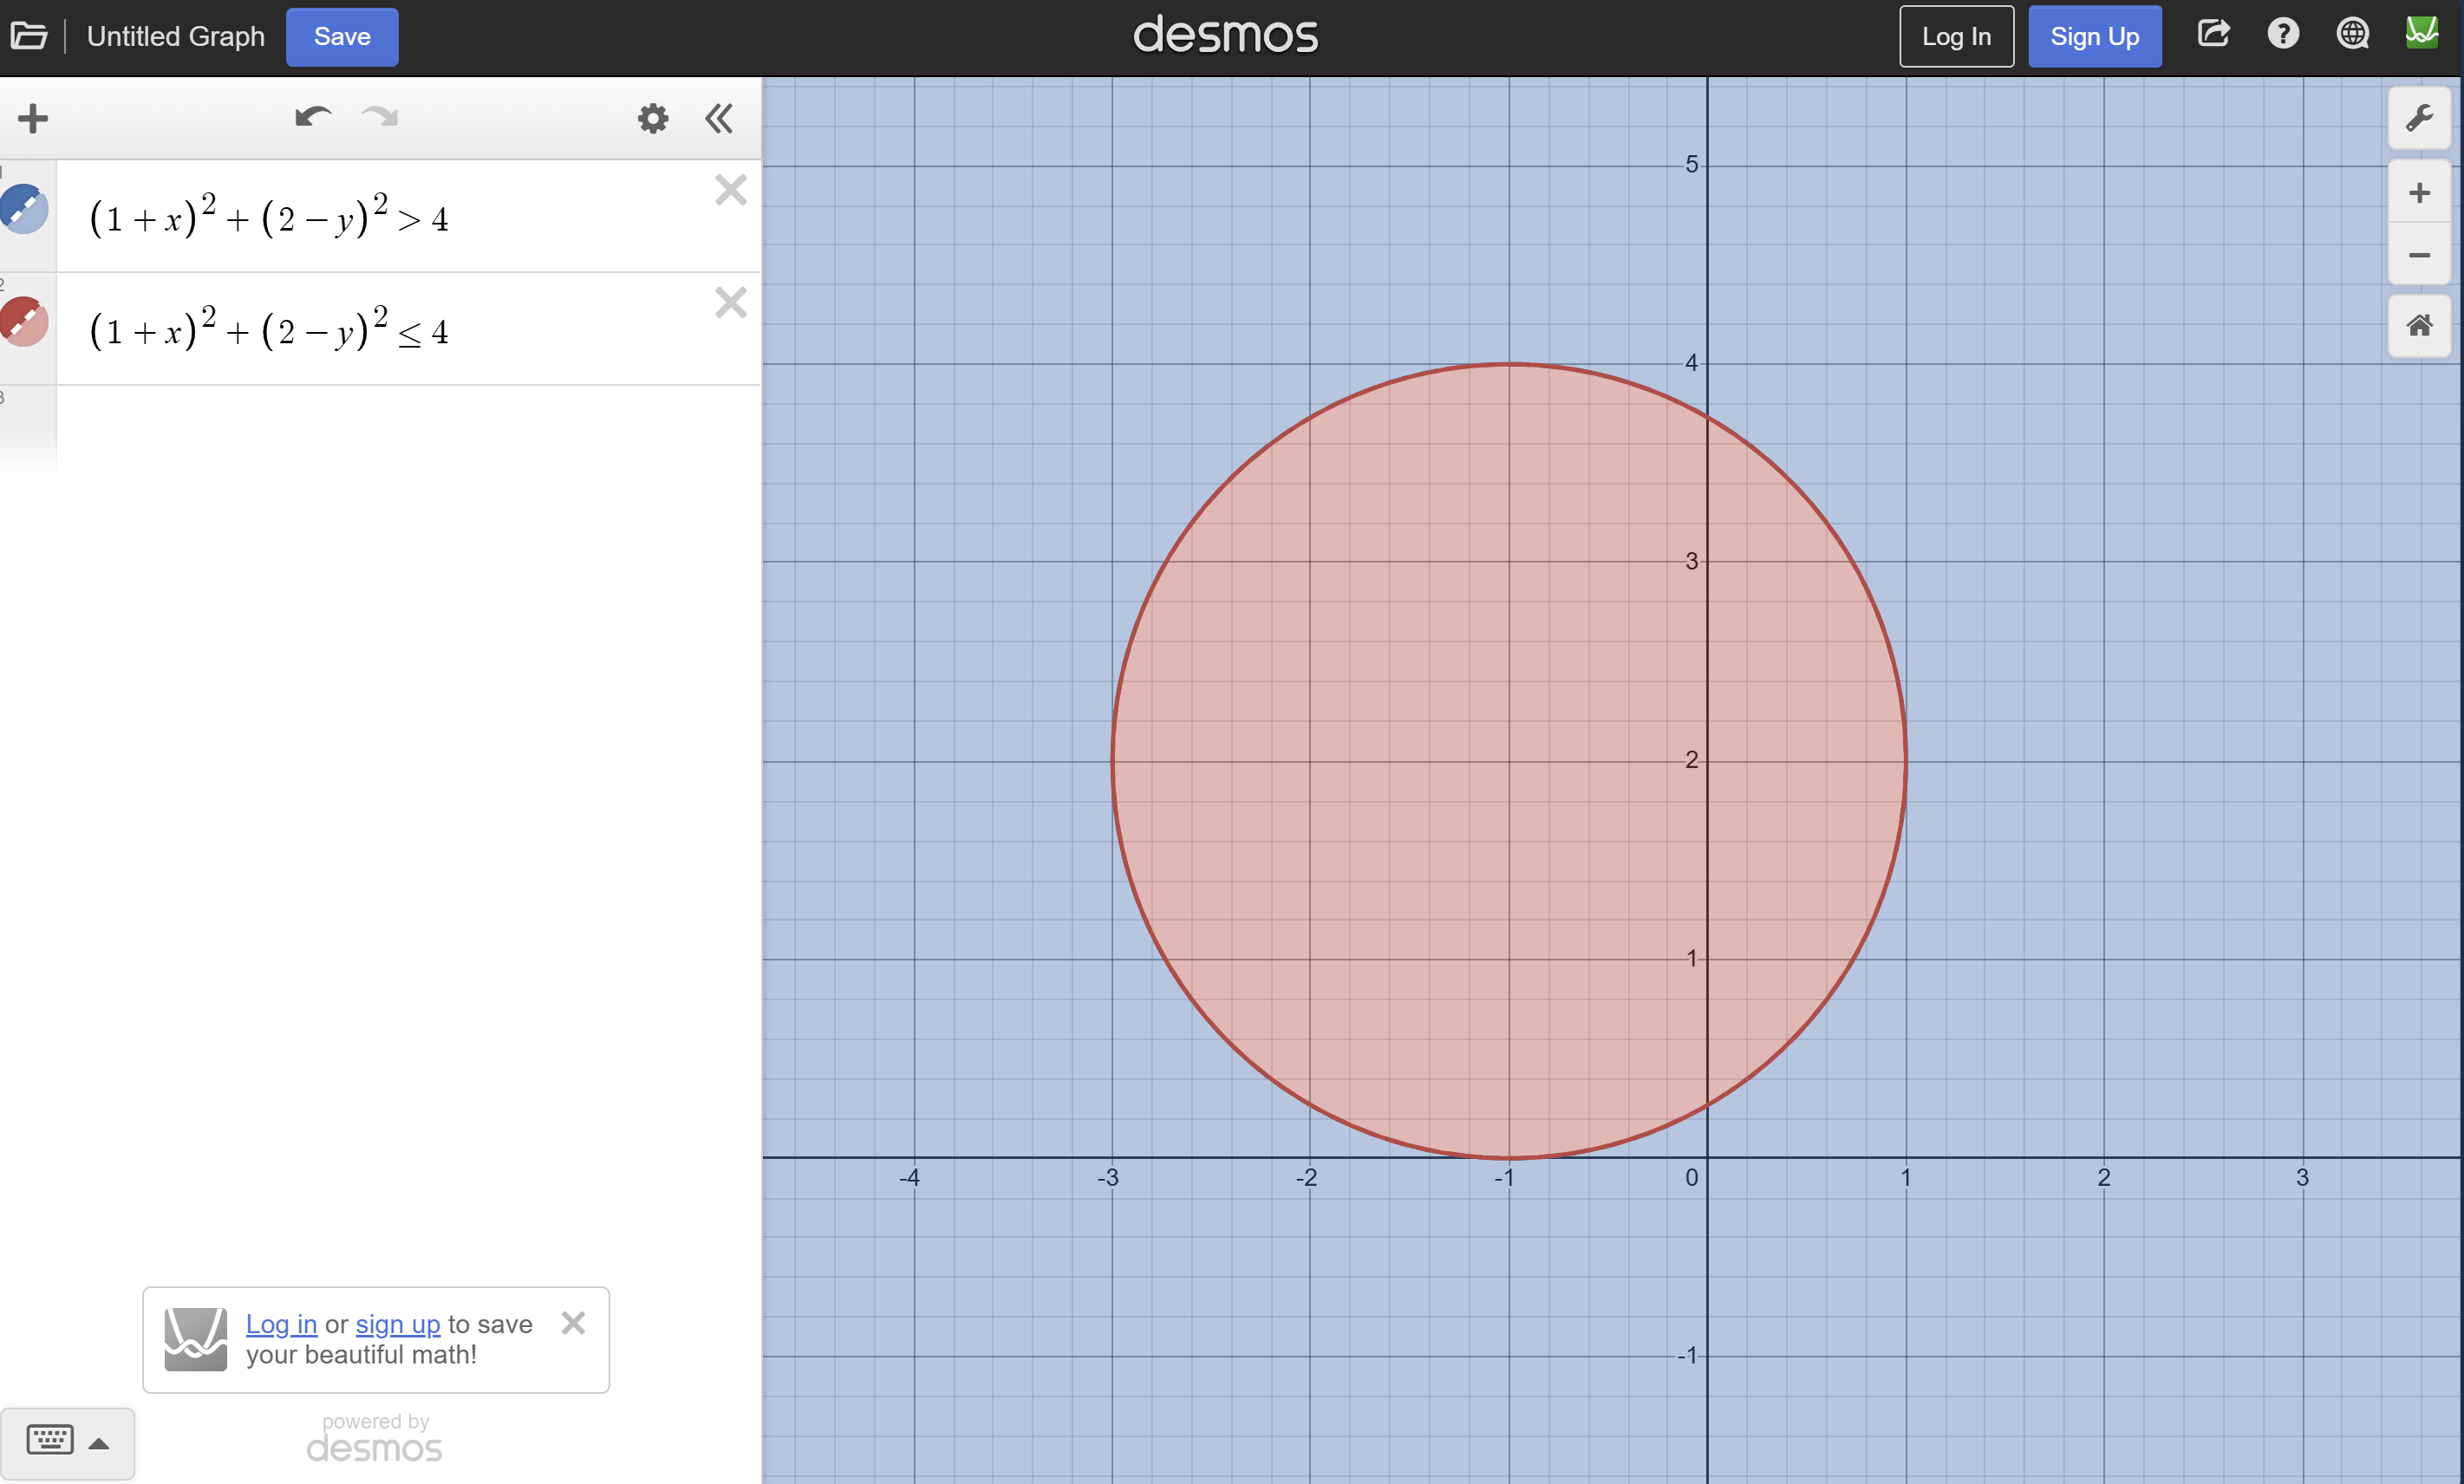
\includegraphics[width=0.5\textwidth]{Images/3b.png}
                \end{center}
                The set of points for which $(1 + X_1)^2 + (2 - X_2)^2 > 4$ is outside the circle (colored blue), and the set of points for which $(1 + X_1)^2 + (2 - X_2)^2 \leq 4$ is inside the circle and the edge (colored red).
            \end{soln}
        \end{subprob}

        \begin{subprob}
            Suppose that a classifier assigns an observation to the blue class if $(1 + X_1)^2 + (2 - X_2)^2 > 4$, and to the red class otherwise. To what class is the observation (0, 0) classified? (-1, 1)? (2, 2)? (3, 8)?

            \begin{soln}
                (0, 0) is classified as blue, (-1, 1) is classified as red, (2, 2) is classified as blue, and (3, 8) is classified as blue.
            \end{soln}
        \end{subprob}

        \begin{subprob}
            Argue that while the decision boundary in (c) is not linear in terms of $X_1$ and $X_2$, it is linear in terms of $X_1, X_2, X_1^2, X_2^2, X_1X_2$.

            \begin{soln}
                The decision boundary is not linear in terms of $X_1$ and $X_2$ because it is a circle. However, it is linear in terms of $X_1, X_2, X_1^2, X_2^2, X_1X_2$ because it can be written as $X_1^2 + X_2^2 + 2X_1 - 4X_2 + 1 = 0$.
            \end{soln}
        \end{subprob}
    \end{subprobset}
\end{prob}

\newpage

\begin{prob}[\textbf{Ch. 9 conceptual exercise 3}]
    Here we explore the maximal margin classifier on a toy data set.

    \begin{subprobset}
        \begin{subprob}
            We are given $n = 7$ observations in $p = 2$ dimensions. For each observation, there is an associated class label.
            
            \begin{center}
                \begin{tabular}{cccc}
                    \hline
                    Obs. & $X_1$ & $X_2$ & $Y$ \\
                    \hline
                    1 & 3 & 4 & Red \\
                    2 & 2 & 2 & Red \\
                    3 & 4 & 4 & Red \\
                    4 & 1 & 4 & Red \\
                    5 & 2 & 1 & Blue \\
                    6 & 4 & 3 & Blue \\
                    7 & 4 & 1 & Blue \\
                    \hline
                \end{tabular}
            \end{center}

            Sketch the observations.

            \begin{soln}
                \begin{center}
                    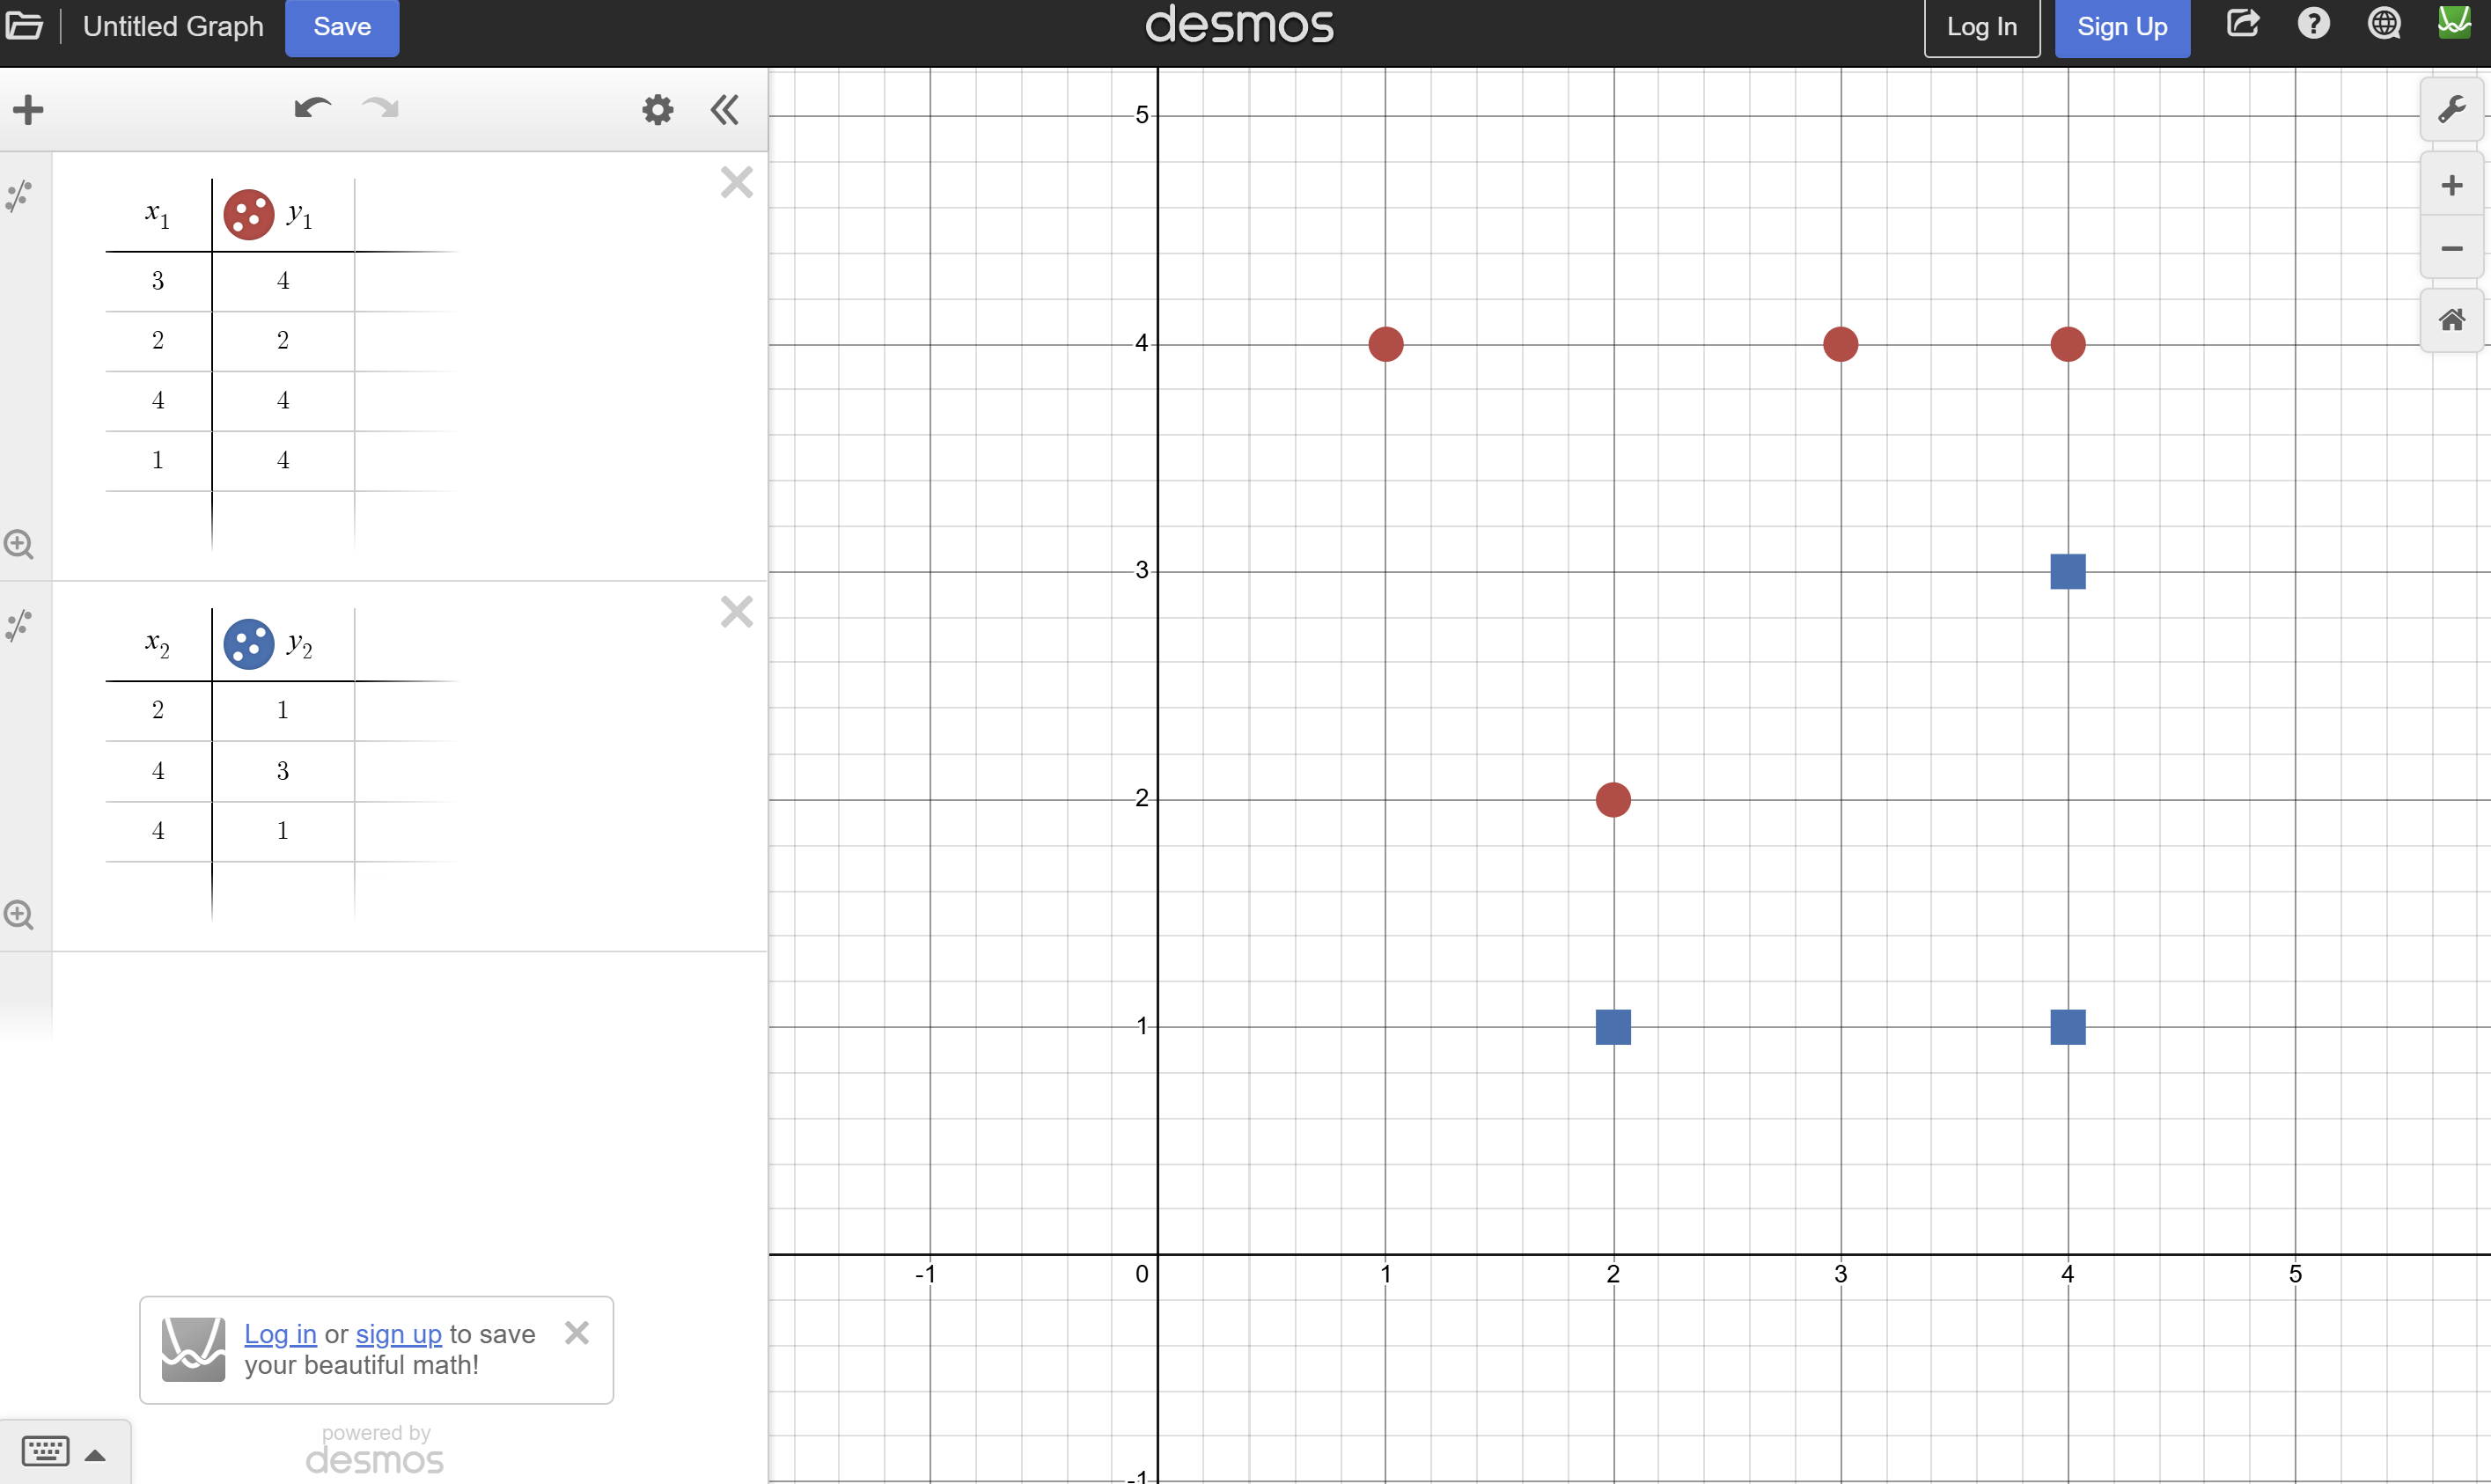
\includegraphics[width=0.5\textwidth]{Images/4a.png}
                \end{center}
            \end{soln}
        \end{subprob}

        \begin{subprob}
            Sketch the optimal separating hyperplane, and provide the equation for this hyperplane.

            \begin{soln}
                \begin{center}
                    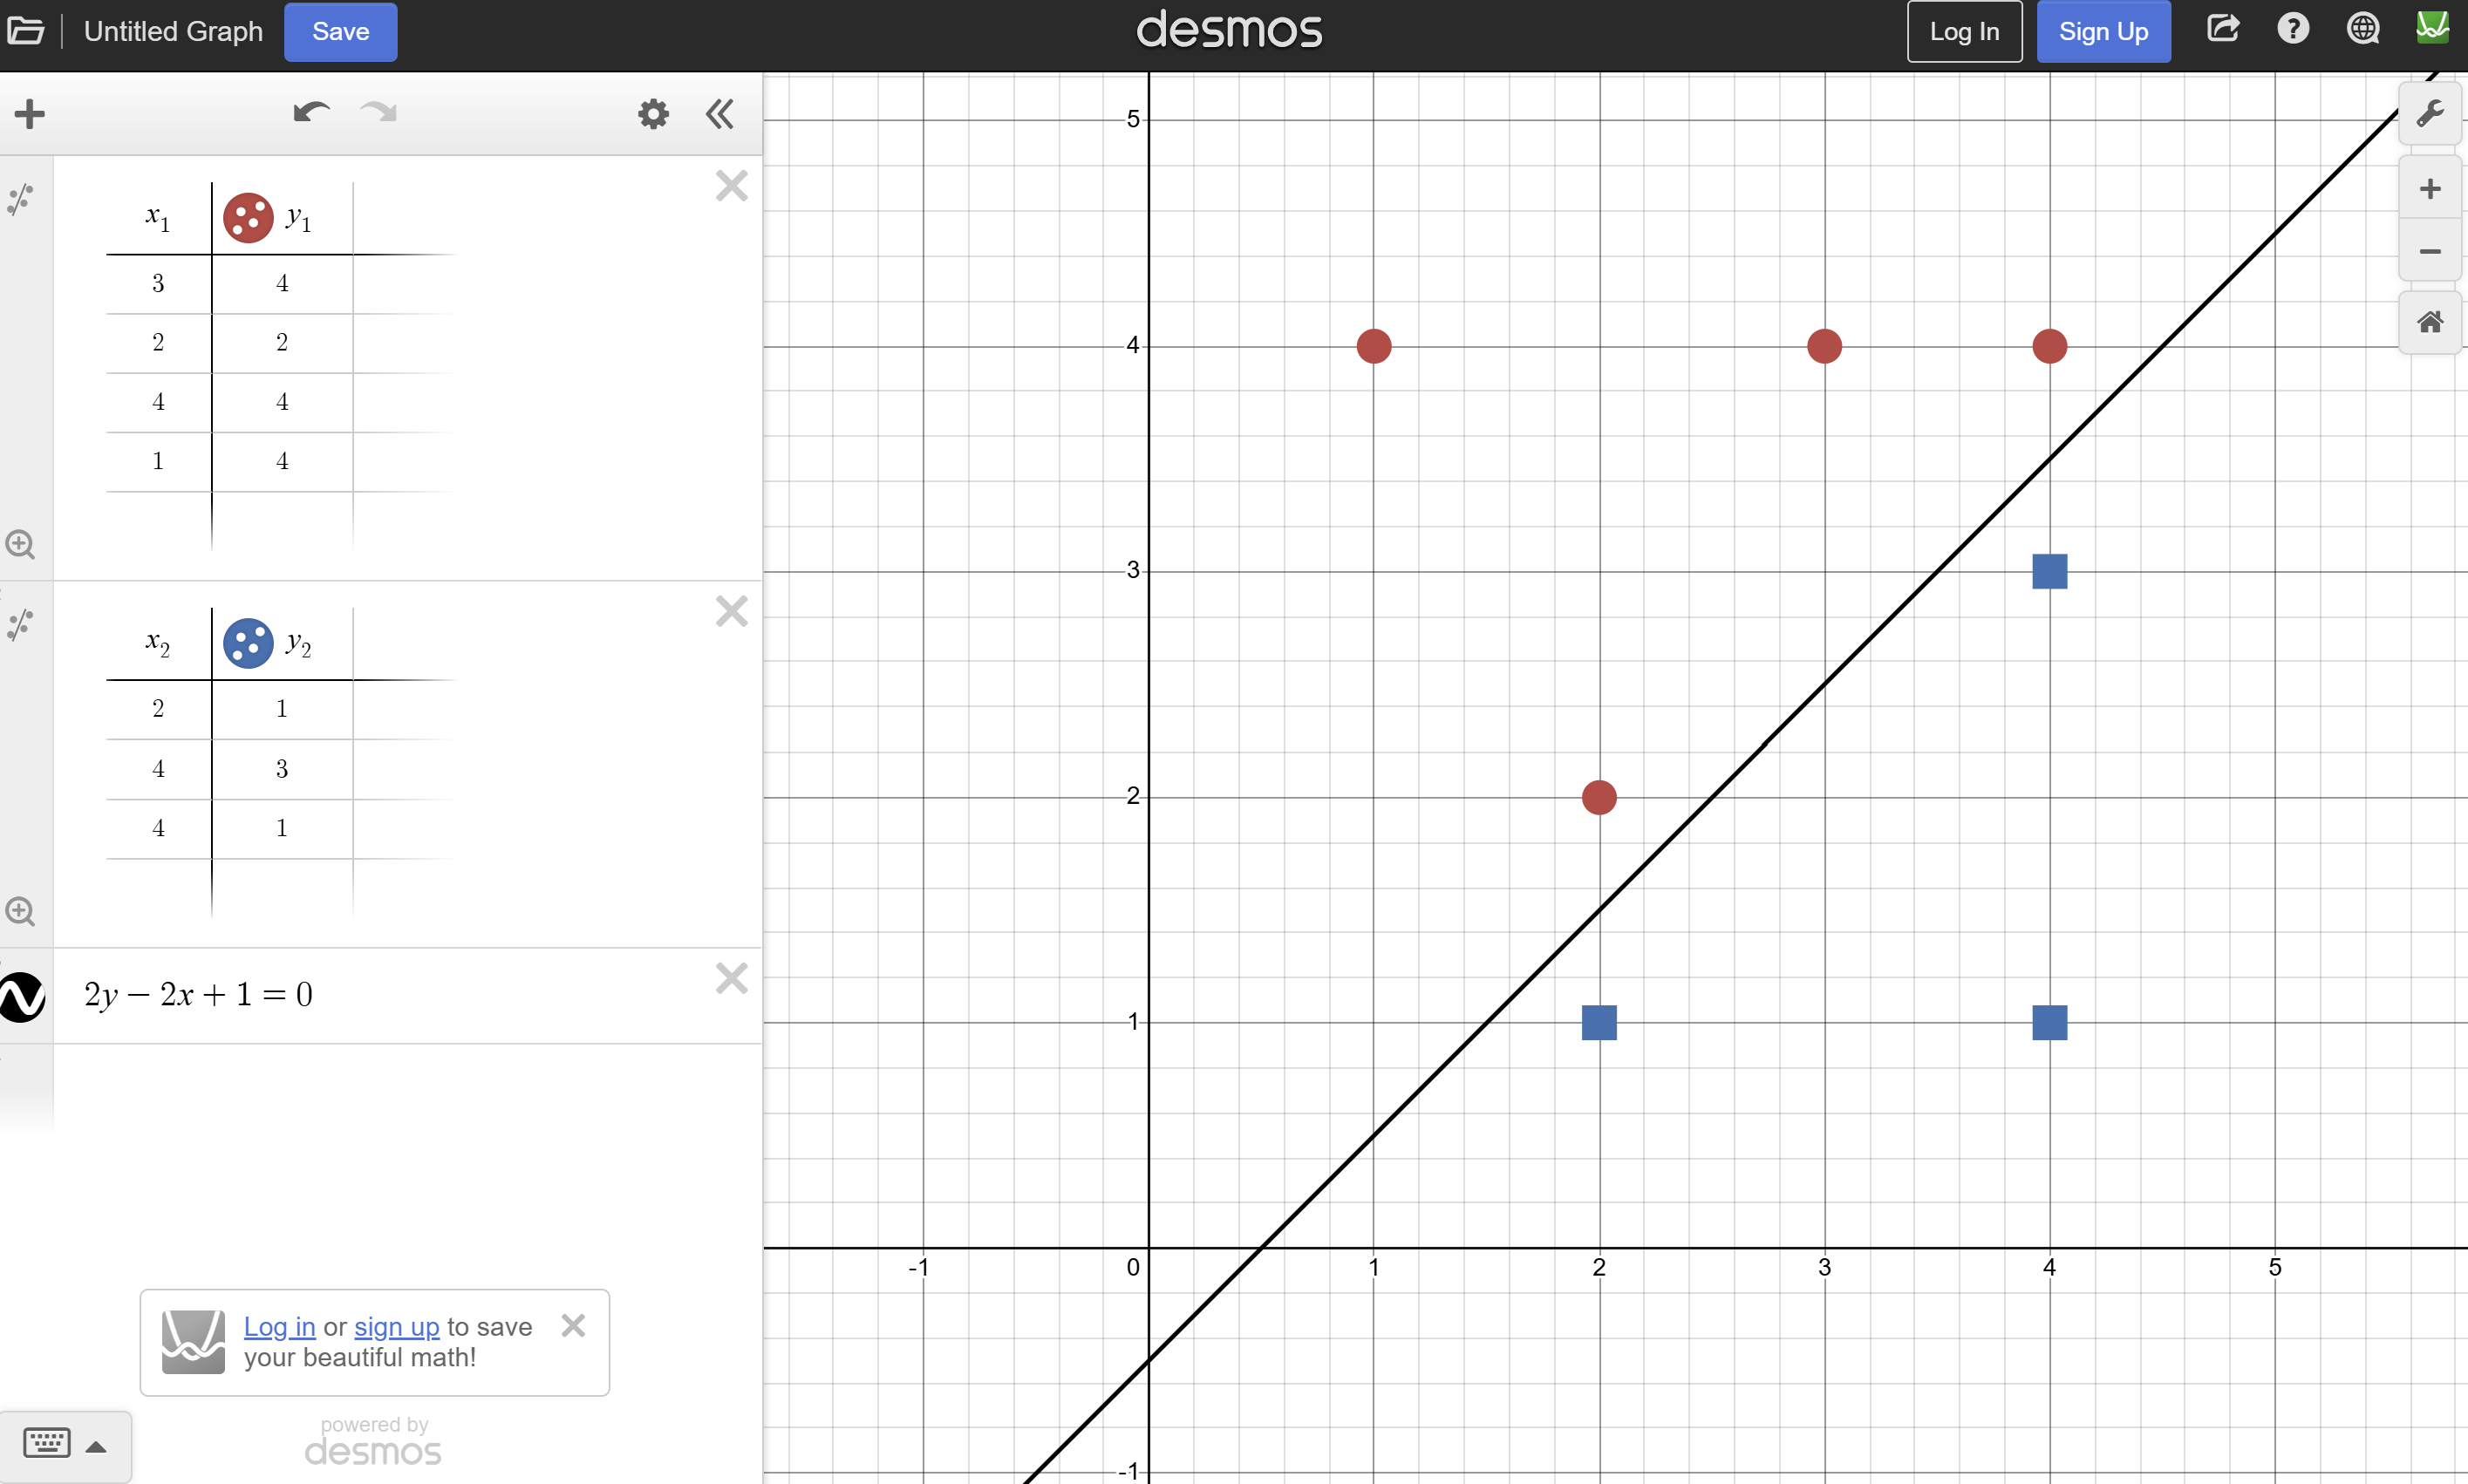
\includegraphics[width=0.5\textwidth]{Images/4b.png}
                \end{center}
                The optimal separating hyperplane is the line that maximizes the margin between the two classes. The equation for this hyperplane is $1 - 2X_1 + 2X_2 = 0$.
            \end{soln}
        \end{subprob}

        \begin{subprob}
            Describe the classification rule for the maximal margin classifier. It should be something along the lines of "Classify to Red if $\beta_0 + \beta_1X_1 + \beta_2X_2 > 0$, and classify to Blue otherwise." Provide the values for $\beta_0$, $\beta_1$, and $\beta_2$.

            \begin{soln}
                Classify to Red if $1 - 2X_1 + 2X_2 > 0$, and classify to Blue otherwise. The values for $\beta_0$, $\beta_1$, and $\beta_2$ are 1, -2, and 2, respectively.
            \end{soln}
        \end{subprob}

        \begin{subprob}
            On your sketch, indicate the margin for the maximal margin hyperplane.

            \begin{soln}
                \begin{center}
                    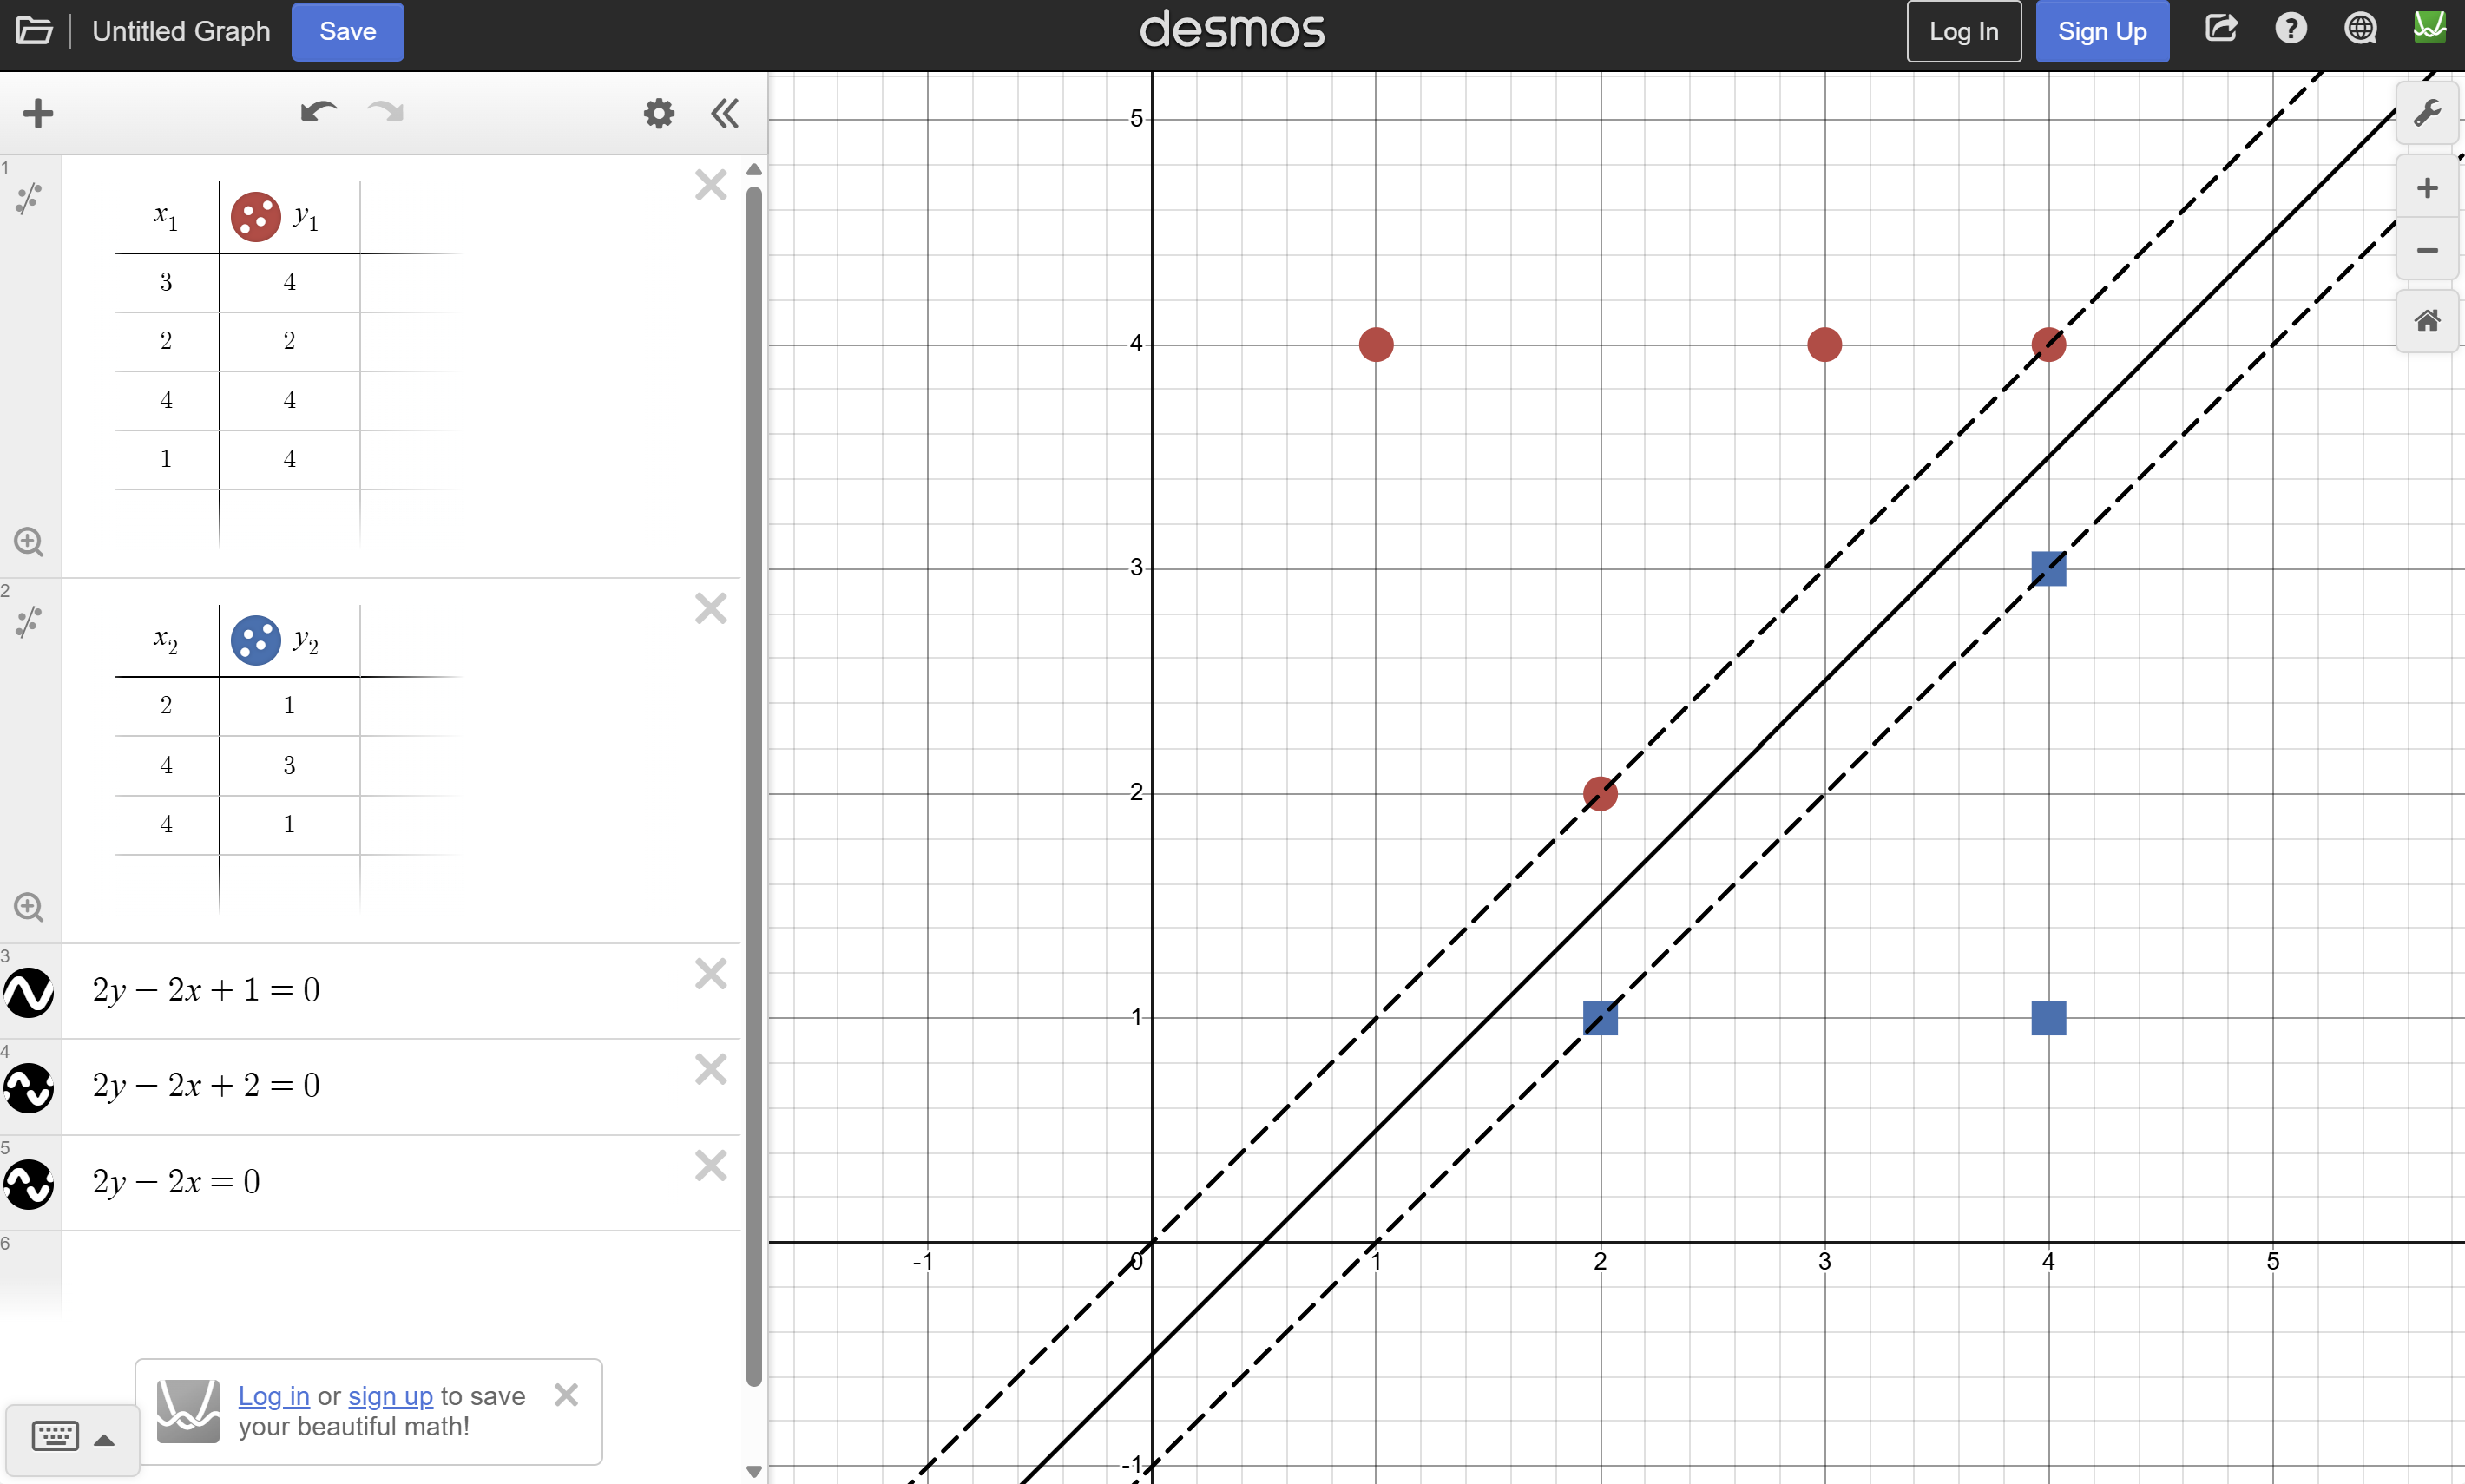
\includegraphics[width=0.5\textwidth]{Images/4d.png}
                \end{center}
            \end{soln}
        \end{subprob}

        \begin{subprob}
            Indicate the support vectors for the maximal margin classifier.

            \begin{soln}
                The support vectors for Red are (2, 2) and (4, 4) while the support vectors for Blue are (2, 1) and (4, 3).
            \end{soln}
        \end{subprob}

        \begin{subprob}
            Argue that a slight movement of the seventh observation would not affect the maximal margin hyperplane.

            \begin{soln}
                A small movement for Obs. 7 wouldn't affect the hyperplane because it is not a support vector.
            \end{soln}
        \end{subprob}

        \begin{subprob}
            Sketch a hyperplane that is not the optimal separating hyperplane, and provide the equation for this hyperplane.

            \begin{soln}
                \begin{center}
                    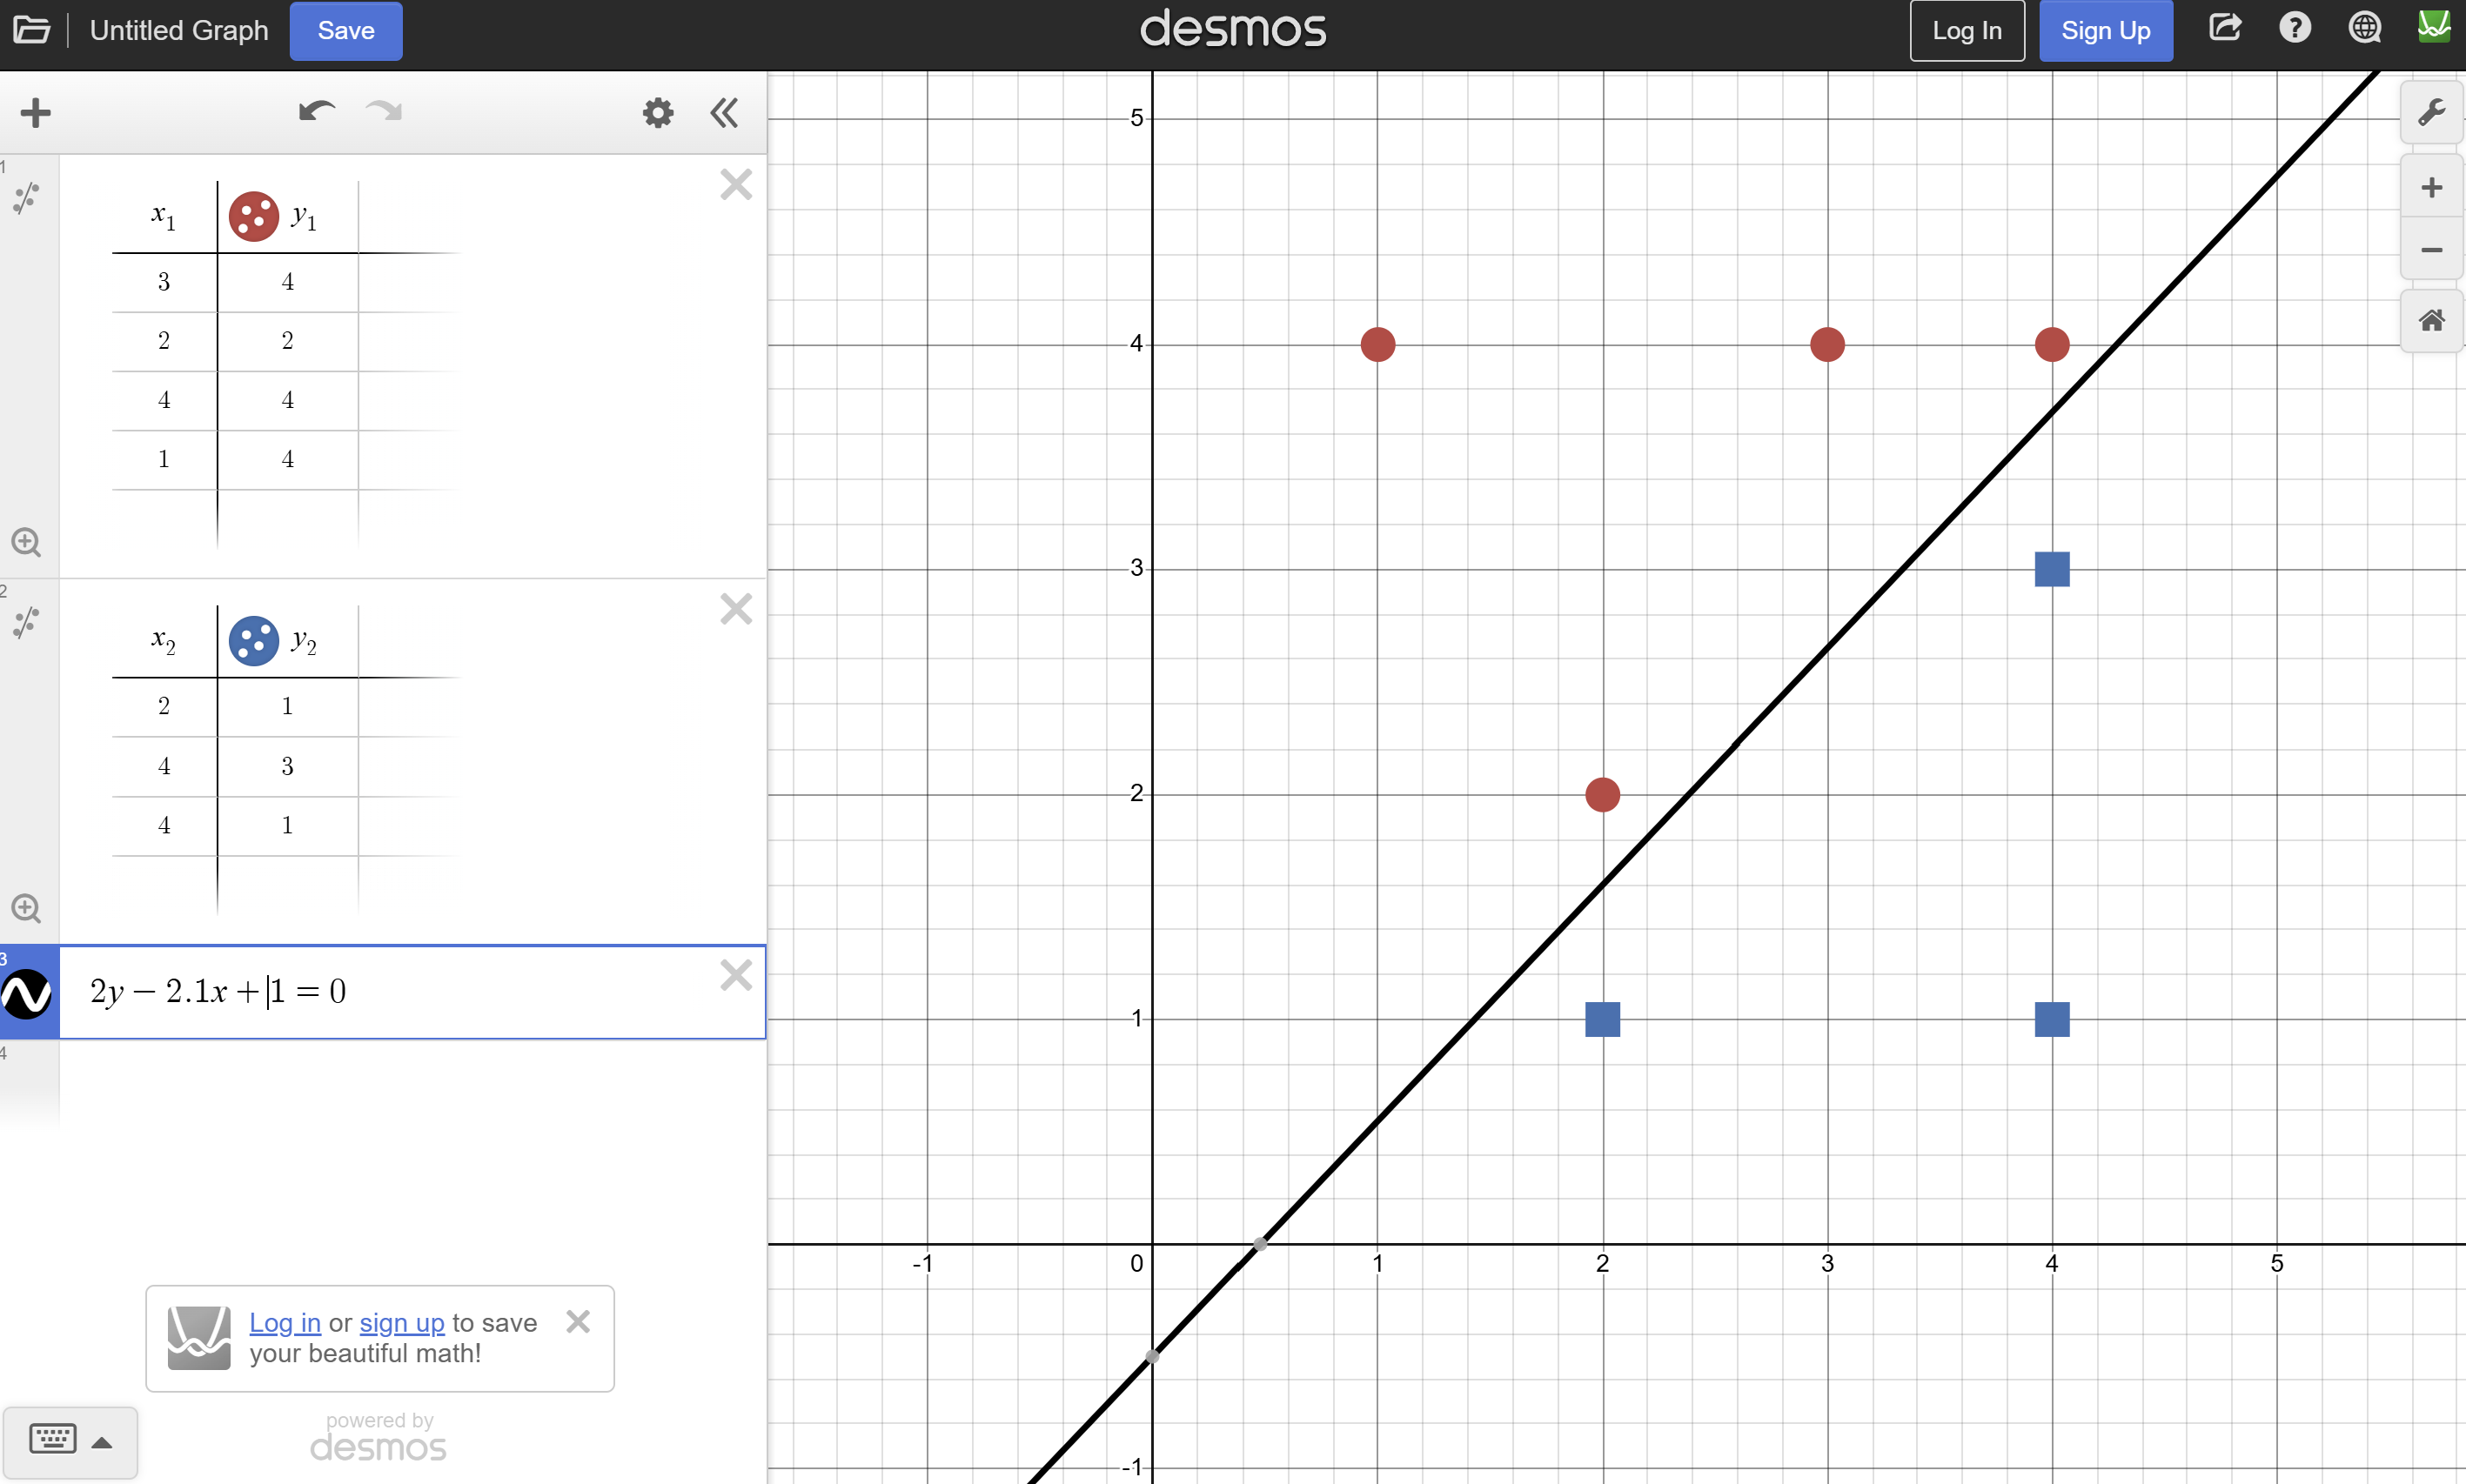
\includegraphics[width=0.5\textwidth]{Images/4g.png}
                \end{center}
                The equation for this hyperplane is $1 - 2.1X_1 + 2X_2 = 0$.
            \end{soln}
        \end{subprob}

        \newpage

        \begin{subprob}
            Draw an additional observation on the plot so that the two classes are no longer separable by a hyperplane.

            \begin{soln}
                \begin{center}
                    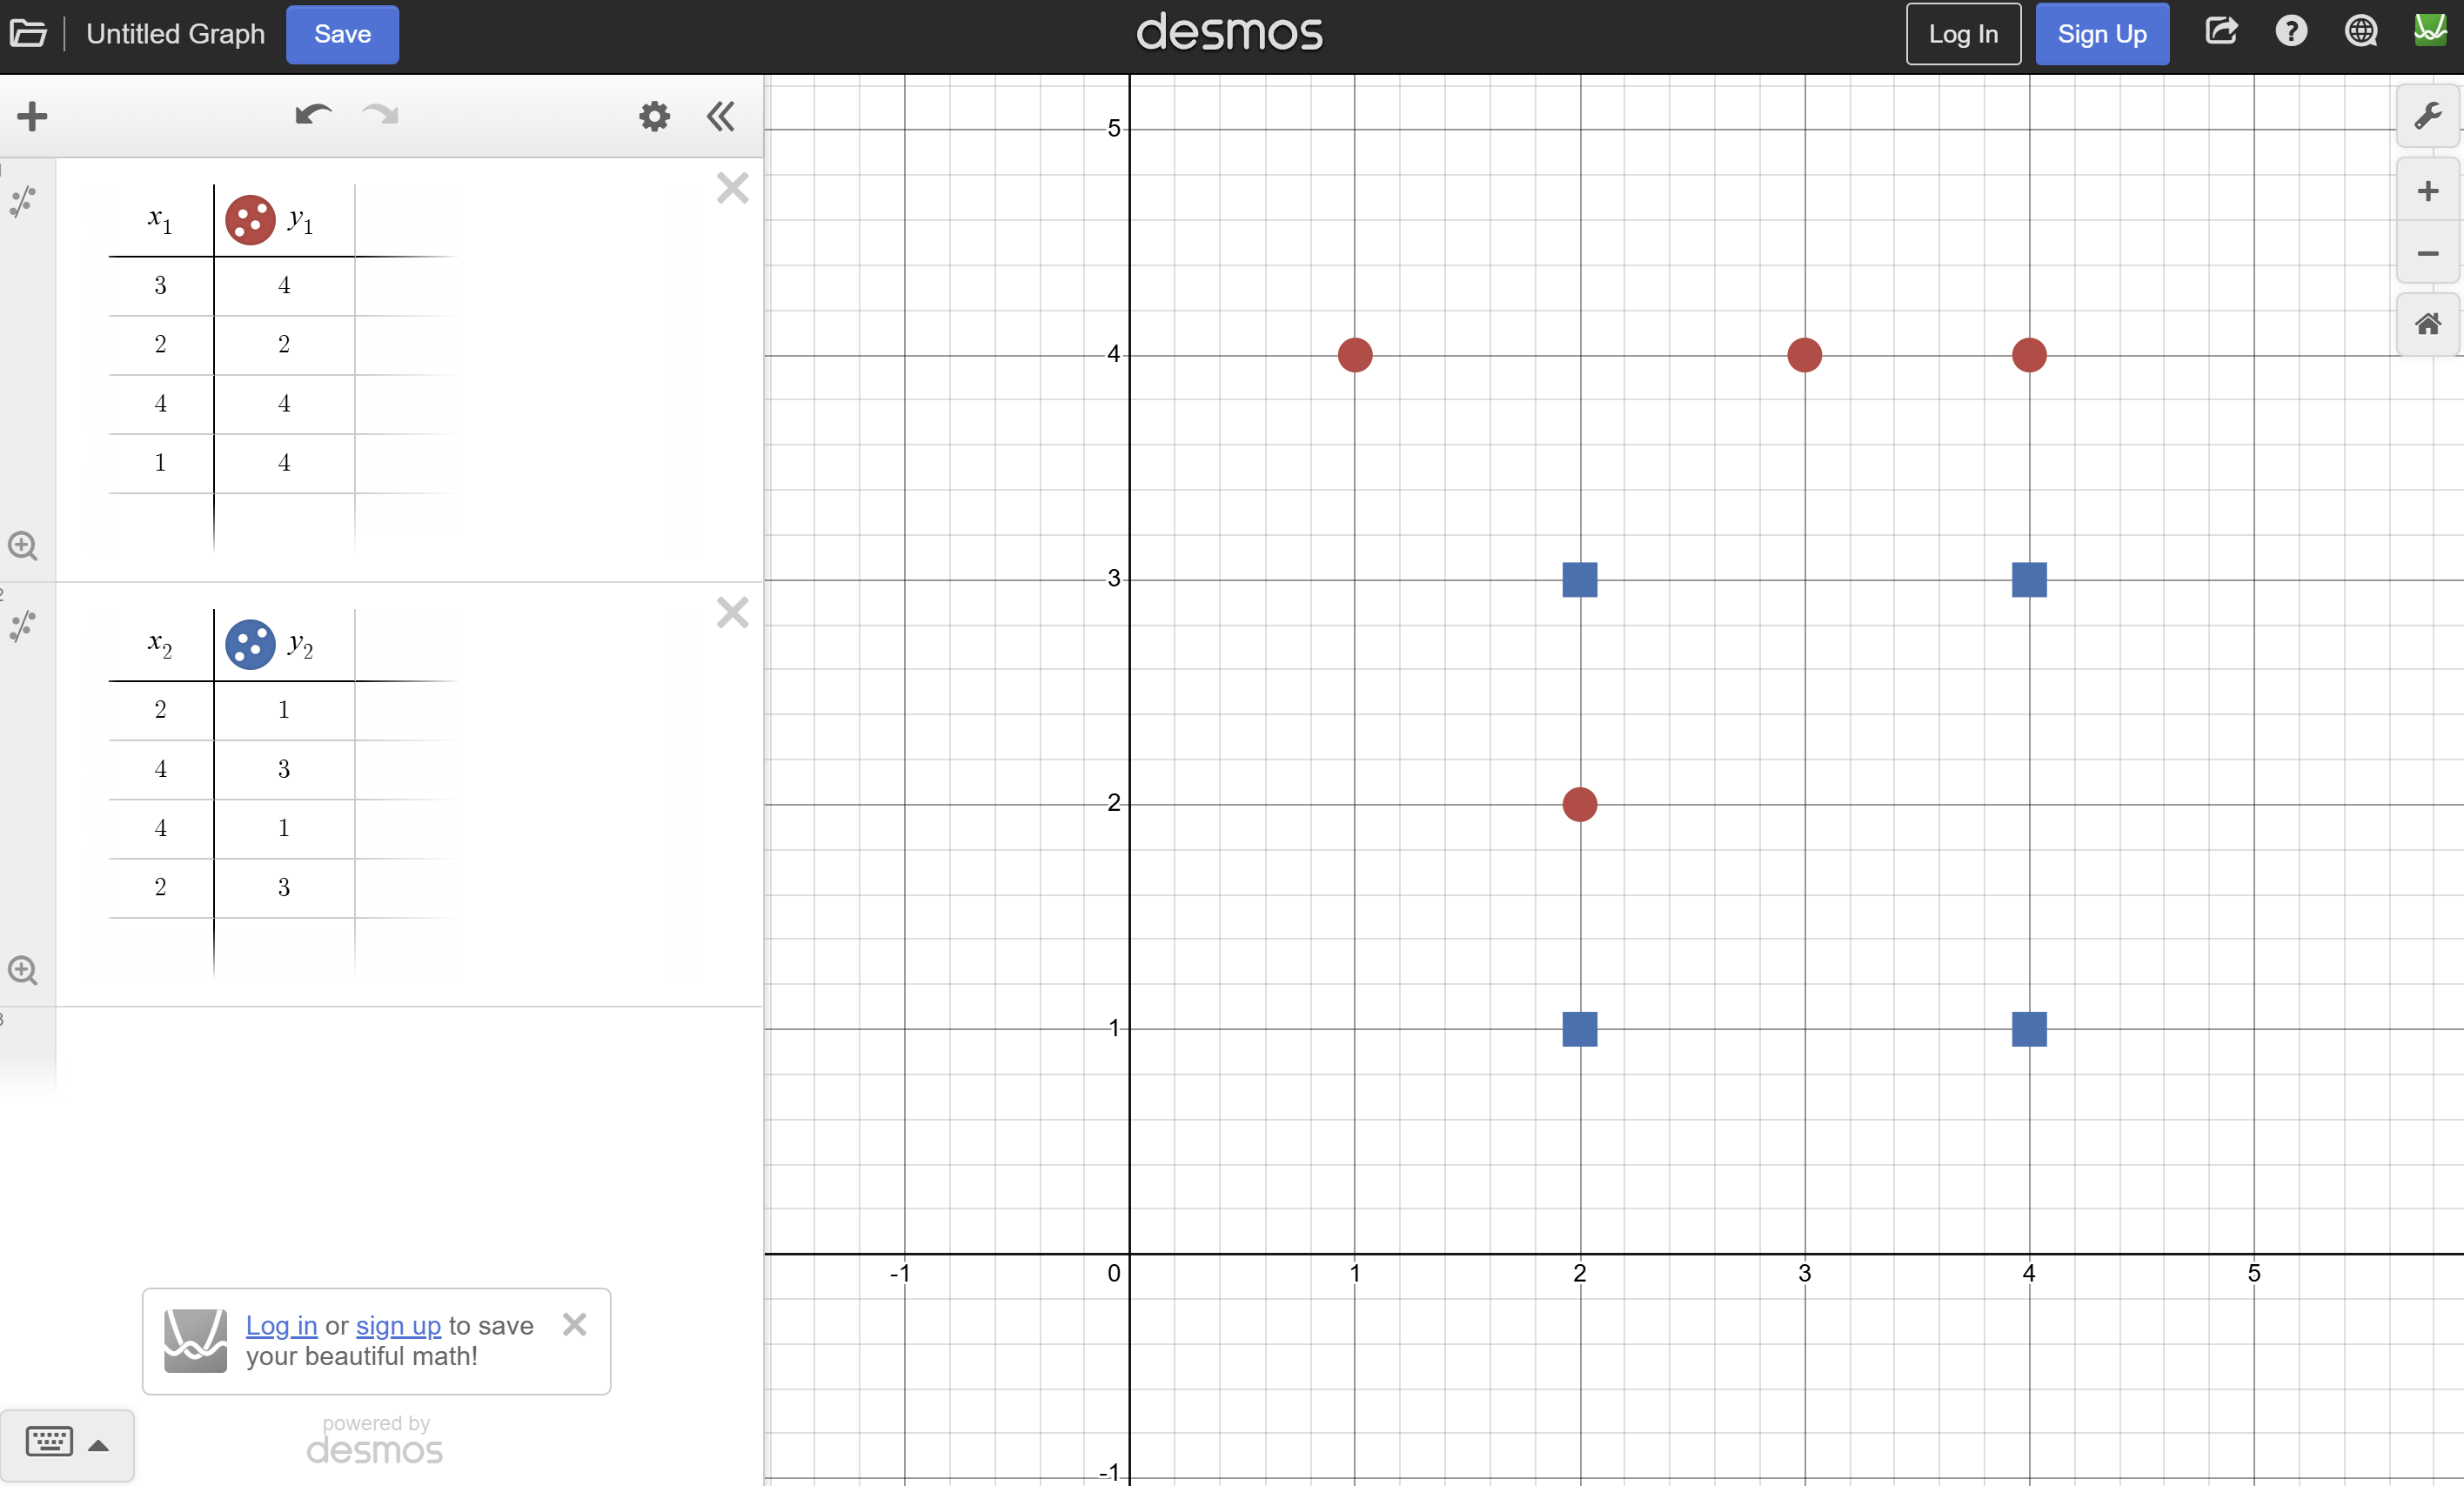
\includegraphics[width=0.5\textwidth]{Images/4h.png}
                \end{center}
                Adding the observation (2, 3) as a Blue point makes the two classes no longer separable by a hyperplane.
            \end{soln}
        \end{subprob}
    \end{subprobset}
\end{prob}

\begin{prob}[\textbf{Ch. 8 applied exercise 8, with part (f) removed.}]
    Using the \texttt{Carseats} data set, we will seek to predict \texttt{Sales} using regression trees and related approaches, treating the response as a quantitative variable.

    \begin{subprobset}
        \begin{subprob}
            Split the data set into a training set and a test set.

            \begin{soln}
                Code is attached to the end.
            \end{soln}
        \end{subprob}

        \begin{subprob}
            Fit a regression tree to the training set. Plot the tree, and interpret the results. What test MSE do you obtain?

            \begin{soln}
                \begin{center}
                    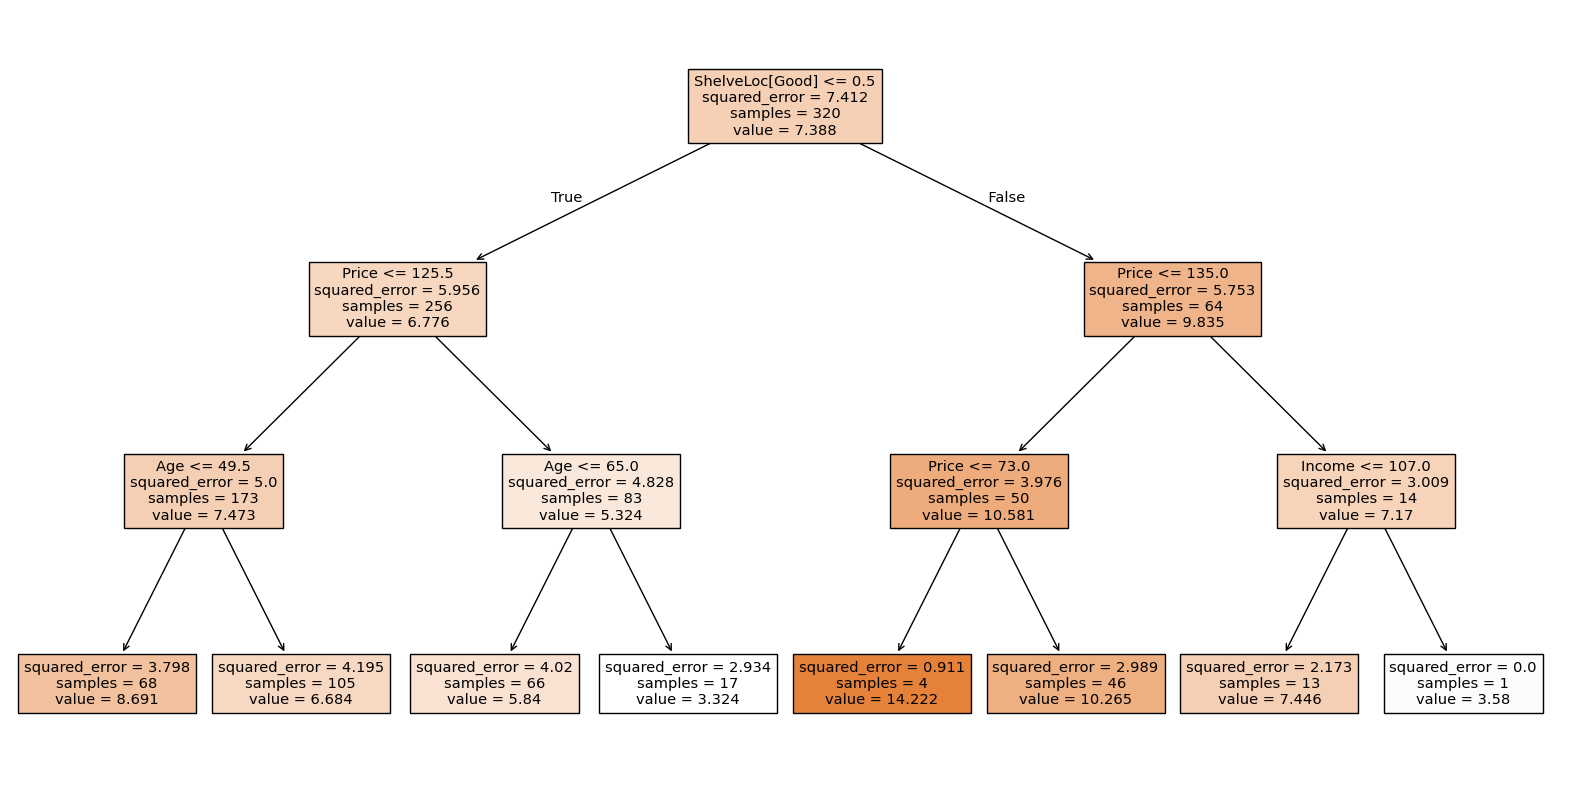
\includegraphics[width=0.5\textwidth]{Images/5b.png}
                \end{center}
                The test MSE is 6.6841. Setting the max depth to 3, we find that the important features are \texttt{ShelveLoc}, \texttt{Price}, \texttt{Age}, and \texttt{Income} since most decisions are made on these features.
            \end{soln}
        \end{subprob}

        \begin{subprob}
            Use cross-validation in order to determine the optimal level of tree complexity. Does pruning the tree improve the test MSE?

            \begin{soln}
                The test MSE for the full tree is 6.0762 and 5.9015 for the pruned tree. From this, we can see that pruning the tree improves the test MSE.
            \end{soln}
        \end{subprob}

        \newpage

        \begin{subprob}
            Use the bagging approach in order to analyze this data. What test MSE do you obtain? Use the \texttt{feature\_ importance\_} values to determine which variables are most important.

            \begin{soln}
                With bagging, we get a test MSE of 3.0638. The top 5 most important features are \texttt{Price}, \texttt{ShelveLoc[Good]}, \texttt{Age}, \texttt{CompPrice}, and \texttt{Advertising} in descending order of importance.
            \end{soln}
        \end{subprob}

        \begin{subprob}
            Use random forests to analyze this data. What test MSE do you obtain? Use the \newline \texttt{feature\_ importance\_} values to determine which variables are most important. Describe the effect of $m$, the number of number of variables considered at each split, on the error rate obtained.

            \begin{soln}
                The test MSE was the same as with bagging at 3.0638. The top 5 most important features are the same as with bagging. The effect of $m$ (max\_features) on test MSE is as follows:
                \begin{itemize}
                    \item $m=1$: Test MSE = 6.0147
                    \item $m=3$: Test MSE = 3.9052
                    \item $m=6$: Test MSE = 3.0847
                    \item $m=11$: Test MSE = 3.0638
                \end{itemize}
                It seems that increasing $m$ decreases the test MSE until it reaches the number of features, at which point the test MSE is the same as with bagging.
            \end{soln}
        \end{subprob}
    \end{subprobset}
\end{prob}

\begin{prob}[\textbf{Ch. 9 applied exercise 4}]
    Generate a simulated two-class data set with 100 observations and two features in which there is a visible but non-linear separation between the two classes. Show that in this setting, a support vector machine with a polynomial kernel (with degree greater than 1) or a radial kernel will outperform a support vector classifier on the training data. Which technique performs best on the test data? Make plots and report training and test error rates in order to back up your assertions.

    \begin{soln}
        \begin{center}
            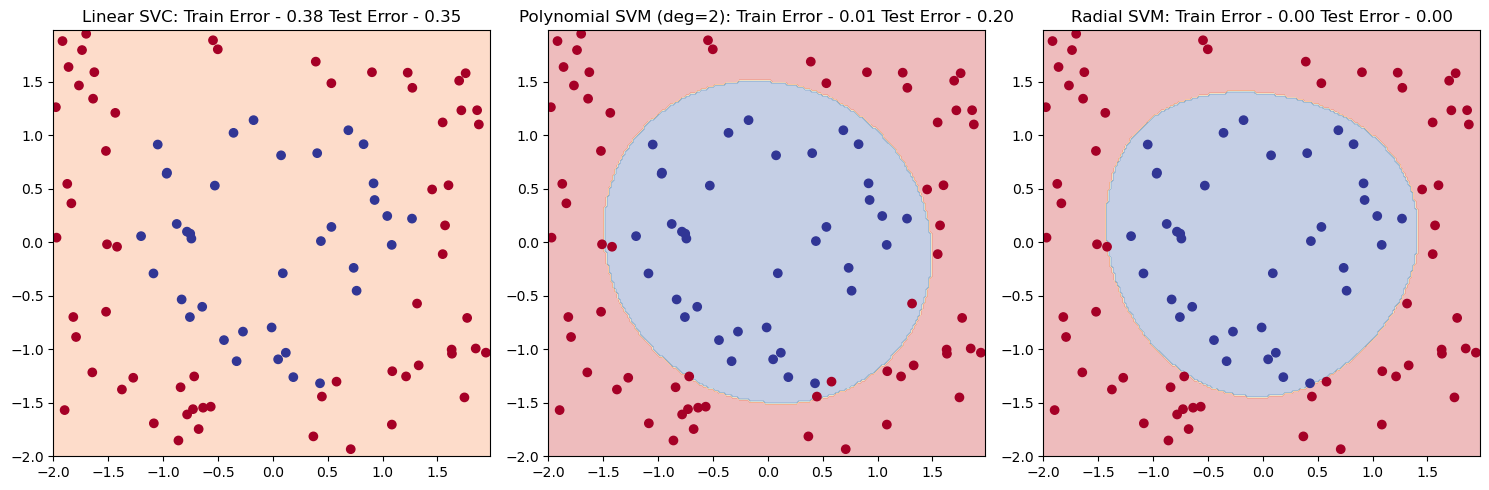
\includegraphics[width=\textwidth]{Images/6.png}
        \end{center}
        I generated the data by sampling 100 points from $(x, y) \in [-2, 2] \times [-2, 2]$ and labeling them as Blue if $x^2 + y^2 \leq 2$ and Red otherwise.
        
        While both the polynomial and radial kernels outperform the linear kernel on the training data, the SVM with the radial kernel performs best on both the training and test data with errors of 0. The linear kernel performs worst on both the training and test data with errors of 0.38 and 0.35, respectively. The polynomial kernel is able to fit the data somewhat, but isn't able to fit perfectly and gets a training error of 0.01 and test error of 0.20.
    \end{soln}
\end{prob}
\end{probset}
\end{document}